\documentclass[11pt]{article}
\usepackage{background,geometry,enumitem,kotex,fancyhdr}

%Change the font
\renewcommand{\familydefault}{\sfdefault}

\pagestyle{fancy}
\fancyhf{}

\rfoot{Page \thepage}
%
\includegraphics{contact}
\definecolor{deepblue}{RGB}{07, 31, 75}
\definecolor{customgrey}{RGB}{117, 117, 117}

\newcommand{\sectionB}[1]{%
    \section*{\textcolor{deepblue}{#1}}%
}


\newcommand{\sectionbox}[3]{%
  \vtop{%
    \subsection*{\textcolor{deepblue}{#1}}%
    \textcolor{deepblue}{#2}
    #3%
  }%
}



%Prevent extra spacing between bullets
\setlist{nolistsep}

%Set geometry to fill the entire page
\geometry{
  total={8.5in,11in},
  textheight=10.5in,
  textwidth=8in,
}

\setlist[itemize]{label=\textcolor{customgrey}{\LARGE\textbullet}}


%Add the background image to each of the resume pages.
\backgroundsetup{
  scale=1,
  angle=0,
  opacity=1,
  contents={
    \ifnum\value{page}>1
      
\includegraphics[width=\paperwidth]{resumebg2}
    \else
      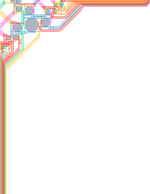
\includegraphics[width=\paperwidth]{resumebg1}
    \fi
  }
}

\begin{document}
\twocolumn[
  \begin{flushright}
    \begin{minipage}{0.5\textwidth}
    \centering
      
\includegraphics{name} \\
      \textcolor{deepblue}{{\small Flattened Version. View the human-friendly version here:}\\
      {\large \textbf{www.noyama-dev.com/resume/}}}
    \end{minipage}
  \end{flushright}
]
\thispagestyle{empty}

\sectionB{Skills}

\sectionbox{Training/Mentoring/Teaching}{Confidence: 90\%}{\\
  I enjoy working in a team setting, and I also enjoy communicating with both technical and non-technical audiences. For example, I have:
  \begin{itemize}
    \item Walked through Proof of Concept software with potential clients
    \item Addressed parents' questions and concerns for a summer programming class
    \item Trained co-workers on how to scrape information using NLP
    \item Mentored interns one-on-one and helped them feel welcome in the workplace
    \item Presented dozens of lectures to 100+ students in a 2-story lecture hall
  \end{itemize}
}


\sectionbox{Statistics/Classifiers}{Confidence: 80\%}{\\
I studied CTMC's for my master's research, and my work at Kingland has encouraged me to learn Naive Bayes classifiers to the point where I can teach it.
  \begin{itemize}
    \item I have implemented a custom Naive Bayes Classifier from scratch that used log-normally distributed, historical trend data
    \item I have implemented, and I understand the math behind Continuous Time Markov Chains
    \item For small models, one can directly solve the steady state
    \item For models too large for memory, I can simulate paths in the model
    \item For more complicated queries, I have experience using the probabilistic model checker, PRISM
  \end{itemize}
}


\sectionbox{Machine Learning}{Confidence: 60\%}{\\
  Through classes and my work at Kingland, I have an awareness of many Machine Learning methods and confidence in a few detailed below. I also understand the math behind neural networks (e.g. the chain rule).
  \begin{itemize}
    \item I have implemented a recurrent neural network using Keras/ Tensorflow
    \item I have read, and I understand academic literature on NLP techniques like word2vec/doc2vec
    \item I have written algorithms to train Naive-Bayes classifiers and derived the most relevant terms using a term-frequency/inverse-window-frequency metric
  \end{itemize}
}


\sectionbox{Natural Language Processing}{Confidence: 70\%}{\\
  I have done a lot of work with the open source NLP library spaCy.
  \begin{itemize}
    \item I've used syntax parse trees to scrape information from data filed with the Securities and Exchange Commision
    \item I've created several heuristics for tying named entities to entities in a structured, relational database
    \item I've investigated using other machine learning techniques for classifying sentences/windows of text
  \end{itemize}
}


\sectionbox{Bioinformatics/Dynamic Prog.}{Confidence: 80\%}{\\
  I have implemented algorithms using Suffix Trees, Tries, maximal cliques and the Longest Common Subsequence problem for general text processing with Kingland Systems. My master's work in DNA nanotechnology introduced me to many of these algorithms.
}


\sectionbox{Design Patterns/Architecture}{Confidence: 80\%}{\\
  I love learning about and applying design patterns for both statically and dynamically typed languages. My favorite books are:
  \begin{itemize}
    \item \emph{Head First Design Patterns} by Bates, Sierra, Freeman and Robson
    \item \emph{Game Programming Patterns} by Nystrom
  \end{itemize}
  My favorite pattern is the composite pattern. One can implicitly use it with maps/dicts, and a surprising number of things work better as trees (e.g. scene-graphs, game entities and ETL processes).
}


\sectionbox{RDBS Design}{Confidence: 60\%}{\\
  I have designed two relational schemas, one for a volunteer project and one for Kingland. I have learned about 1st/2nd/3rd and Boyce-Codd Normal Form, and I am confident I can design sensible schemas with referential integrity.
}

\begin{center}
\includegraphics[height = 2cm]{contact}\end{center}

\sectionbox{Technical Writing/Publishing}{Confidence: 60\%}{\\
  For both my bachelor's and master's degrees I wrote a 70 page thesis. I have also authored one conference paper and co-authored another. I have received compliments for my documentation at work (though that's proprietary ;P). Bibliography:
  \begin{itemize}
    \item Nakayama, Brian. \emph{Modeling Technologies and Methods for DNA Origami}. Diss. Iowa State University, 2016.
    \item Thein Than Tun, Robyn Lutz, Brian Nakayama, Yijun Yu, Divita Mathur and Bashar Nuseibeh. ``The role of environmental assumptions in failures of DNA nanosystems," COUFLESS 2015, Florence, Italy. ACM, 2015.
    \item Nakayama, Brian and Bahr, David, ``Universal Computation in the Prisoner's Dilemma Game," UCNC 2014, London, Ontario. Springer: Lecture Notes in Computer Science, 2014.
    \item Nakayama, Brian. \emph{Universal Computation in the Prisoner's Dilemma Game}. Diss. Regis University, 2013.
  \end{itemize}
}


\sectionB{Languages/Tools}

\sectionbox{Java}{Confidence: 90\%}{\\
  I started teaching myself Java in 2006 before my junior year in highschool. I have since taught others how to program in Java as an instructor for two sections of an undergraduate course titled ``Introduction to Object Oriented Programming" (COMS 227), and as an instructor for three sections of a highschool summer course titled ``Computer Science: Program Your Own Game." While at Kingland, I use Java $\sim$25\% of the time.
}


\sectionbox{Python}{Confidence: 80\%}{\\
I first used Python to create plugins for DNA Origami CAD software. At Kingland, Python is the primary language I use, and I prefer it for its conciseness and my productivity. However, for speed and traceability, statically typed languages (such as Java) often make more sense. I've worked with the following libraries/APIs:
\begin{itemize}
  \item \textbf{spaCy}: Natural Language Processing
  \item \textbf{numpy}: Linear Algebra
  \item \textbf{sciPy}: Statistics and ML
  \item \textbf{flask/gunicorn}: REST Framework
  \item \textbf{cython}: C-Extensions for CPython
  \item \textbf{boto3}: AWS API

\end{itemize}
}


\sectionbox{PostgreSQL/Flyway}{Confidence: 60\%}{\\
  \begin{itemize}
    \item I have installed, setup and used Postgres for RDBS.
    \item I use psql to manually run queries and pgpsql to create server side functions.
    \item I have used \emph{explain/analyze} commands to find missing indices.
    \item I have set up cron jobs to vaccuum the database to increase efficiency.
    \item I have installed and used Flyway to incrementally design schemas.
  \end{itemize}
}


\sectionbox{Linux/Bash/Shell}{Confidence: 60\%}{\\
  Whenever I don't know how to use a command, I think \emph{man}, if only there was a way to look up what it does? Needless to say, I know just enough to be snarky, but not enough to not use Google! Usually I can get by using a \emph{.bashrc} file to predefine those pesky PATHs and other commands I have a tough time remembering. I also enjoy Vim, though I have successfully avoided Emacs for quite some time.
}


\sectionbox{AWS/Cloud/Terraform}{Confidence: 60\%}{\\
  Amazon Web Services consists of over 90 services. Of those services, I have used the following:
  \begin{itemize}
    \item Web Console
    \item Elastic Cloud Compute (EC2) instances
    \item EC2 Container Service/Repo (ECS/ECR)
    \item Elastic File System (EFS)
    \item Elastic Search (Not AWS specific)
    \item Elastic/Application Load Balancers (ELB/ALB)
    \item Terraform/Infrastructure as Code
    \item Jenkins/Continuous Deployments
  \end{itemize}
  I have also tinkered or helped with the following:
  \begin{itemize}
    \item IAM policies
    \item Ansible
    \item DynamoDB
    \item API Gateway
  \end{itemize}
  Please contact me if you have specific questions about my AWS experience.
}

\begin{center}
\includegraphics[height = 2cm]{logo}\end{center}

\sectionbox{Containers/Docker}{Confidence: 50\%}{\\
  I have made and deployed docker containers on AWS ECS clusters. I have created custom containers for Postgres, Airflow, and Python based Natural Language Processing services using a \emph{Dockerfile}. I have also created custom build contexts by using a script to generate <i>.dockerignore</i> files. Though I still have much to learn in this area, I recognize its power, and I believe this will continue to be important in the future. (I would like to learn more about Container Orchestration Engines in the future.)
}


\sectionbox{Git/Version Control}{Confidence: 70\%}{\\
  {\LaTeX}  is a scripting language that one can use to create beautiful and interactive PDFs. If I needed to make an important presentation, or if I wanted to write a patent, I would use {\LaTeX}  to do this. I wrote many homework assignments, most of my lectures and all of my published papers using \LaTeX. I also use Standard Vector Graphics for hand coded images.
}


\sectionbox{Javascript/JQuery}{Confidence: 70\%}{\\
  When I first learned Javascript, back in 2006, people still had to worry about making their web pages compatible with Netscape, flash was still a thing, and people used ``Dynamic HTML" to update the Document Object Model. As a language, Javascript has a lot of similarities with Python, despite all the curly braces. I made most of the animations on my personal webpage using Javascript to manipulate the DOM of SVG elements, with some help from JQuery where possible to help with transitions and selecting elements.
}


\sectionbox{CSS/SASS}{Confidence: 50\%}{\\
  I do not have encyclopedic knowledge of all of the properties one can manipulate with CSS, but I do at least understand the difference between margins and padding. This website shows what I can do with CSS, including some custom, tailored, responsive design.
}


\sectionbox{C/C++/Golang/Other}{Confidence: 40\%}{\\
  Mostly to see what all the hype was about, I used C++ to write:
  \begin{itemize}
    \item A program for approximating the surface area of protein molecules that implements a deterministic algorithm for evenly distributing points on a sphere
    \item A global sequence alignment algorithm for matching approximately similar pieces of DNA (or any type of string)
  \end{itemize}

  I've also dabbled in other languages:
  \begin{itemize}
    \item I've used C with the Java Native Interface to write a proof of concept code for rendering a cube using only integer arithmetic
    \item I've used both Verilog and VHDL to program Field Programmable Gate Arrays
    \item I recently picked up Golang, for which I am attempting to implement a balancing Bounding Volume Hierarchy
  \end{itemize}
}

\sectionB{Work History}

\sectionbox{Kingland Systems}{Software Engineer\\ 1/2016 - Now}{\\
  A small-medium sized company that specializes in creating software solutions to help large companies comply with regulations mostly in the financial industry. Notable accomplishments include:
  \begin{itemize}
    \item Creating proof-of-concept code and demoing for clients, who eventually signed a large, multi-year contract
    \item Implementing Natural Language Processing and Bioinformatics algorithms to scrape information from unstructured data
    \item Deploying microservices accessed via ALBs using Terraform, and a Docker Container that mounts an AWS EFS drive that runs integration tests via Gauge in AWS ECS
    \item Interviewing full-time ML/AI candidates, and presenting/training internally
    \item Interviewing/Mentoring interns, and presenting on behalf of Kingland on campus and at recruiting events
  \end{itemize}
}

\sectionbox{ISU CS Department}{Instructor\\ 5/2015 - 6/2015, 1/2017 - 5/2017}{\\
  For the Computer Science Department at ISU I taught two sections of Introduction to Object Oriented Programming, one during the summer of 2015 (30 students), and one during the fall of 2017 (150 students) while also working at Kingland. Go to \textbf{www.noyama-dev.com/resume/} to view an example lecture, students reviews and example homeworks.
}

\sectionbox{ISU CS Department}{Research Assistant\\ 6/2013 - 8/2013, 5/2014 - 6/2014, 8/2014 - 4/2015}{\\
  As a research assistant at Iowa State University, I worked on how to apply concepts from Computer Science and Graph theory to model a method for creating nano-scale machines called DNA Origami. I received some publications and gave some presentations on my work.\\

  \textbf{Papers/Presentations}
  \begin{itemize}
    \item Nakayama, Brian. \emph{Modeling Technologies and Methods for DNA Origami}. Diss. Iowa State University, 2016.
    \item Thein Than Tun, Robyn Lutz, Brian Nakayama, Yijun Yu, Divita Mathur and Bashar Nuseibeh. ``The role of environmental assumptions in failures of DNA nanosystems," COUFLESS 2015, Florence, Italy. ACM, 2015.
    \item ``Universal Computation in the Prisoner's Dilemma Ga-me," UCNC 2014, London, Ontario. Springer: Lecture Notes in Computer Science, 2014.
    \item ``DNA Nanotechnology: The Programmable Building Bl-ock of Life," Computer Seminar Series. Simpson College: Simpson, IA.
  \end{itemize}
}

\sectionbox{ISU CS Department}{Teaching Assistant\\ 9/2013 - 4/2014, 8/2015 - 12/2015}{\\
  As a teaching assistant I graded, helped students and gave lectures for the following classes:

  \begin{itemize}
    \item COMS 321: Computer Architectures
    \item COMS 409/509: Computer Architectures
  \end{itemize}
}

\sectionbox{Table 2 Table}{Volunteer Android Dev.\\ 2/2015 - 4/2016}{\\
  While attending graduate school, I volunteered to make an Android application for a food rescue organization called Table to Table. Through this I learned a bit about Android development, and I also managed and advised an undergraduate whom we hired to also work on the app. During this opportunity, I worked closely with Professor Shweta Chopra.
}


\begin{center}\vspace*{0.5cm}
\includegraphics[height = 2cm]{logo}\\\vspace*{0.5cm}

\includegraphics[height = 2cm]{contact}\end{center}

\sectionB{Education}

\sectionbox{Iowa State University}{Ames, IA\\ Master's Comp Sci\\ GPA: 3.89, 6/2013 - 1/2016}{\\
  I became a better inventor, researcher and teacher at ISU. (See my online resume for an unofficial transcript.)\\

  \textbf{Honors/Activities}
  \begin{itemize}
    \item Robert Stewart Early Research Award
    \item Teaching Excellence Award
    \item Pragmatics Fellowship
    \item Graduate Academic Committee Member
    \item Graduate and Professional Student Senator
    \item Computational Thinking Competition Volunteer/Judge
    \item Youth and Shelter Services GRIP Mentor
  \end{itemize}
}

\sectionbox{Regis University}{Denver, CO\\ Bachelor's in Comp Sci, Math\\ Minor in Women's Studies\\ GPA: 3.96, 8/2009 - 5/2013}{\\
  I found my love for Computer Science and Social Justice at Regis. (See my online resume for an unofficial transcript.)\\

  \textbf{Honors/Activities}
  \begin{itemize}
    \item Diversity Award
    \item Math-Science Scholarship
    \item Frederick T. Daly S.J. Award for Excellence in Mathematics
    \item Alan M. Turing Award for Excellence in Computer Science
    \item Honors Program
    \item Multicultural Awareness Committee
    \item President of Gay Straight Alliance
    \item Volunteer at Comfort Caf\'{e}
  \end{itemize}
}

\sectionbox{Korea University}{Seoul, South Korea\\ Study Abroad\\ 2/2012 - 6/2012}{\\
  I learned a lot about myself in Korea, and I picked up some Korean: 저는 브라연 노야마예요. 만나서 반가워요!\\

  \textbf{Highlights from Seoul}
  \begin{itemize}
    \item I met many Korean people, as well as folks from Turkey, the EU, Japan, China, and all over the USA
    \item I met my partner, whom I recently married, in Seoul
    \item I learned about how my upbringing in the USA affects how I interact with others in the wider world.
    \item The immense respect for education in Korea inspired me to go to graduate school
  \end{itemize}
}

\begin{center}
 \textbf{This r\'{e}sum\'{e} was compiled using \LaTeX.}
\end{center}
\end{document} 
